\documentclass[conference]{IEEEtran}
\usepackage{microtype,mathtools,amsmath,multibib,amsfonts,multicol,array,multirow,place ins,cite,makecell,algorithm,algorithmic,subfigure,paralist,graphicx}
%\usepackage{flushend}

\usepackage[font=small,labelfont=bf]{caption}

\usepackage{xspace}
\usepackage{color}
\usepackage{ifthen}
\usepackage{url}
\usepackage{fancybox}


\graphicspath{{zu/}}
\DeclareGraphicsExtensions{.pdf,.jpeg,.png}
\hyphenation{op-tical net-works semi-conduc-tor}


\begin{document}
\title{Title}

\author{
\IEEEauthorblockN{Thai Pangsakulyanont\IEEEauthorrefmark{1}, Patanamon Thongtanunam\IEEEauthorrefmark{2},  Daniel Port\IEEEauthorrefmark{3}, Hajimu Iida\IEEEauthorrefmark{2}}
\\
\IEEEauthorblockA{
\IEEEauthorrefmark{1} Kasetsart University, Thailand\\
@ku.ac.th
}

\IEEEauthorblockA{
\IEEEauthorrefmark{2} Nara Institute of Science and Technology, Japan\\
patanamon-t@is.naist.jp, iida@itc.naist.jp\\
}

\IEEEauthorblockA{
\IEEEauthorrefmark{3} University of Hawaii at Manoa, USA\\
dport@hawaii.edu \\
}
}


\maketitle
\newboolean{showcomments}
\setboolean{showcomments}{true} % toggle to show or hide comments
\ifthenelse{\boolean{showcomments}}
{\newcommand{\nbnote}[2]{
  % \fbox{\bfseries\sffamily\scriptsize#1}
  \fcolorbox{blue}{yellow}{\bfseries\sffamily\scriptsize#1}
  {\sf\small\textit{#2}}
  % \marginpar{\fbox{\bfseries\sffamily#1}}
 }
}
{\newcommand{\nbnote}[2]{}
 \newcommand{\version}{}
}
\newcommand\pick[1]{\nbnote{Pick sez}{\textcolor{magenta}{#1}}}
\newcommand\thai[1]{\nbnote{Thai sez}{\textcolor{blue}{#1}}}


\begin{abstract}

% the freeform style of modern code review

% some comments are not technically contributing


\begin{IEEEkeywords}
Modern Code Review, Software Quality, Text Mining
\end{IEEEkeywords}
\end{abstract}

\section{Introduction}
Software code review is an established method regarded as a best practice in Software Engineering to achieve a sufficient quality in software project. This method mainly intend to early identify defect before integrating changes. The formal inspection\cite{Fagan:1976:DCI:1661010.1661012} is a traditional technique for code review with well-defined structure.
Due to cumbersome process mandating a well-preparation and in-person meetings of the formal inspection, Modern Code Review (MCR)\cite{Bacchelli2013a}, less formal and lightweight code reviews have received much attention nowadays and  put into software development regularly in both industrial and OSS projects. A major difference between MCR and inspection is the in-person meeting is not required in MCR. Reviewers can discuss to find defects by comments through code review tool or mailing list. Then, developers will fix their changes following those comments.

As the performance of code review straight forward to the quality of software project, many studies investigated the influencing factors in both formal inspection\cite{Porter1998,Kemerer2009} and MCR\cite{Baysal2001,Mcintosh,Beller,Hamasaki2013}. However, very little research investigate that in MCR, how does a discussion for a proposed change impact to the software quality. Since most of the proposed change improvements are triggered from reviewer comments \cite{Beller}. McIntosh et. al. \cite{Mcintosh} also found that components which were reviewed without discussion are likely to contain bugs. However, there is a study found that reviewers of MCR in Microsoft only focus on minor logic error rather than discussing deeper \cite{Bacchelli2013a}. As MCR is a lightweight code review, reviewers are not required to strictly examine the proposed code changes as in the formal inspection. 
From prior works, we conjecture that comments of reviewers can be either positively contribute the proposed changes or a discussion which is out of scope.

To understand the impact of discussion in MCR, a manual classification is required as study of Beller et. al. \cite{Beller}. As a massive amount of changes and comments in MCR history\cite{Balachandran2013}, it is painstaking and time consuming to classify data sets to perform quantitative analysis. Moreover, the comments in MCR is unstructured natural text unlike a checklist in the formal inspection. 
%\pick{Need some connection. Says that Massive amount of commits and comment it would be expensive to manually identify. It's natural language }

In this paper, we present an approach to automatically classify the usefulness of comments. We define that the usefulness is a comment that contribute to improve the proposed changes. In our approach, we analyze the similarity between commit message of the proposed changes and their comments. Our key idea is that useful comments are likely to contain similar topic as the proposed changes. To do so, we use text mining techniques, Vector Space Model (VSM) to calculate similarity and use euclidian distance to calculate dissimilarity. 
We create our predictive model by estimating a set of similarity and dissimilarity values that best discriminate between a useful and useless comments using the prediction evaluations: Precision, Recall and F-measure.

For our empirical study, we used a review history of Gerrit\footnote{https://code.google.com/p/gerrit/} system which is tool for supporting MCR process. Our case study project is Qt\footnote{http://qt-project.org/}, a open source project of a cross-platform application and UI framework supported by Digia corporation. To validate our approach, we manually classify the usefulness for 320 comments and measure its accuracy. We also used our predictive model for the all set of comments to preliminary estimate quality of reviews. According to this, we address the following two research questions:

\noindent \textbf{RQ1:} Can we identify useful and useless discussions in code review?\\
\noindent \textbf{RQ2:} Do code reviewers intensively discuss on the proposed changes?

\noindent The main contribution of this paper are:
\begin{itemize}
\item We propose an approach to mine natural text of comments in code reviews and classify their usefulness.
\item The experimental results show that our approach can classify comments with XX of F-measure.
\item We found that XX\% of comments for each review are classified as useful comments, while XX \% of comments are classified as useless comments.
\end{itemize} 
%Software Inspection is basically composed of a three-step procedure: preparation, inspection meeting, and repair.

%Motivation Example.\thai{Wow}


\section{Background}
\subsection{Modern Code Review}
\subsection{Text Mining Techniques}
\subsubsection{tf--idf}
\subsubsection{Similarity Measure}
\subsection{Evaluation Techniques}
\subsubsection{Precision and Recall}
\subsubsection{F-measure}


\section{Classification Method}

% where we got the data
We used the review data sets of the Qt project collected by Hamasaki et al TODO(cite properly).
Only reviews in the master branch of \texttt{qtbase} project are considered,
as it is the most active branch.

% quick structure
Each change includes a \emph{commit message} which describes what is changed.
After a change is submitted to Gerrit, reviewers can give scores to it.
The scores will determine whether the change will be accepted or not.
Reviewers can also add comments to the change, which may optionally be added to a specific line of code inside a changed file.
Majority of the comments are automatically generated by Gerrit and do not contain any user-written text.
In this paper, we use the term \emph{document} to refer to a single commit message or comment.
Fig. \ref{fig:hierarchy} shows the relation between documents.

\begin{figure}[h]
\centering
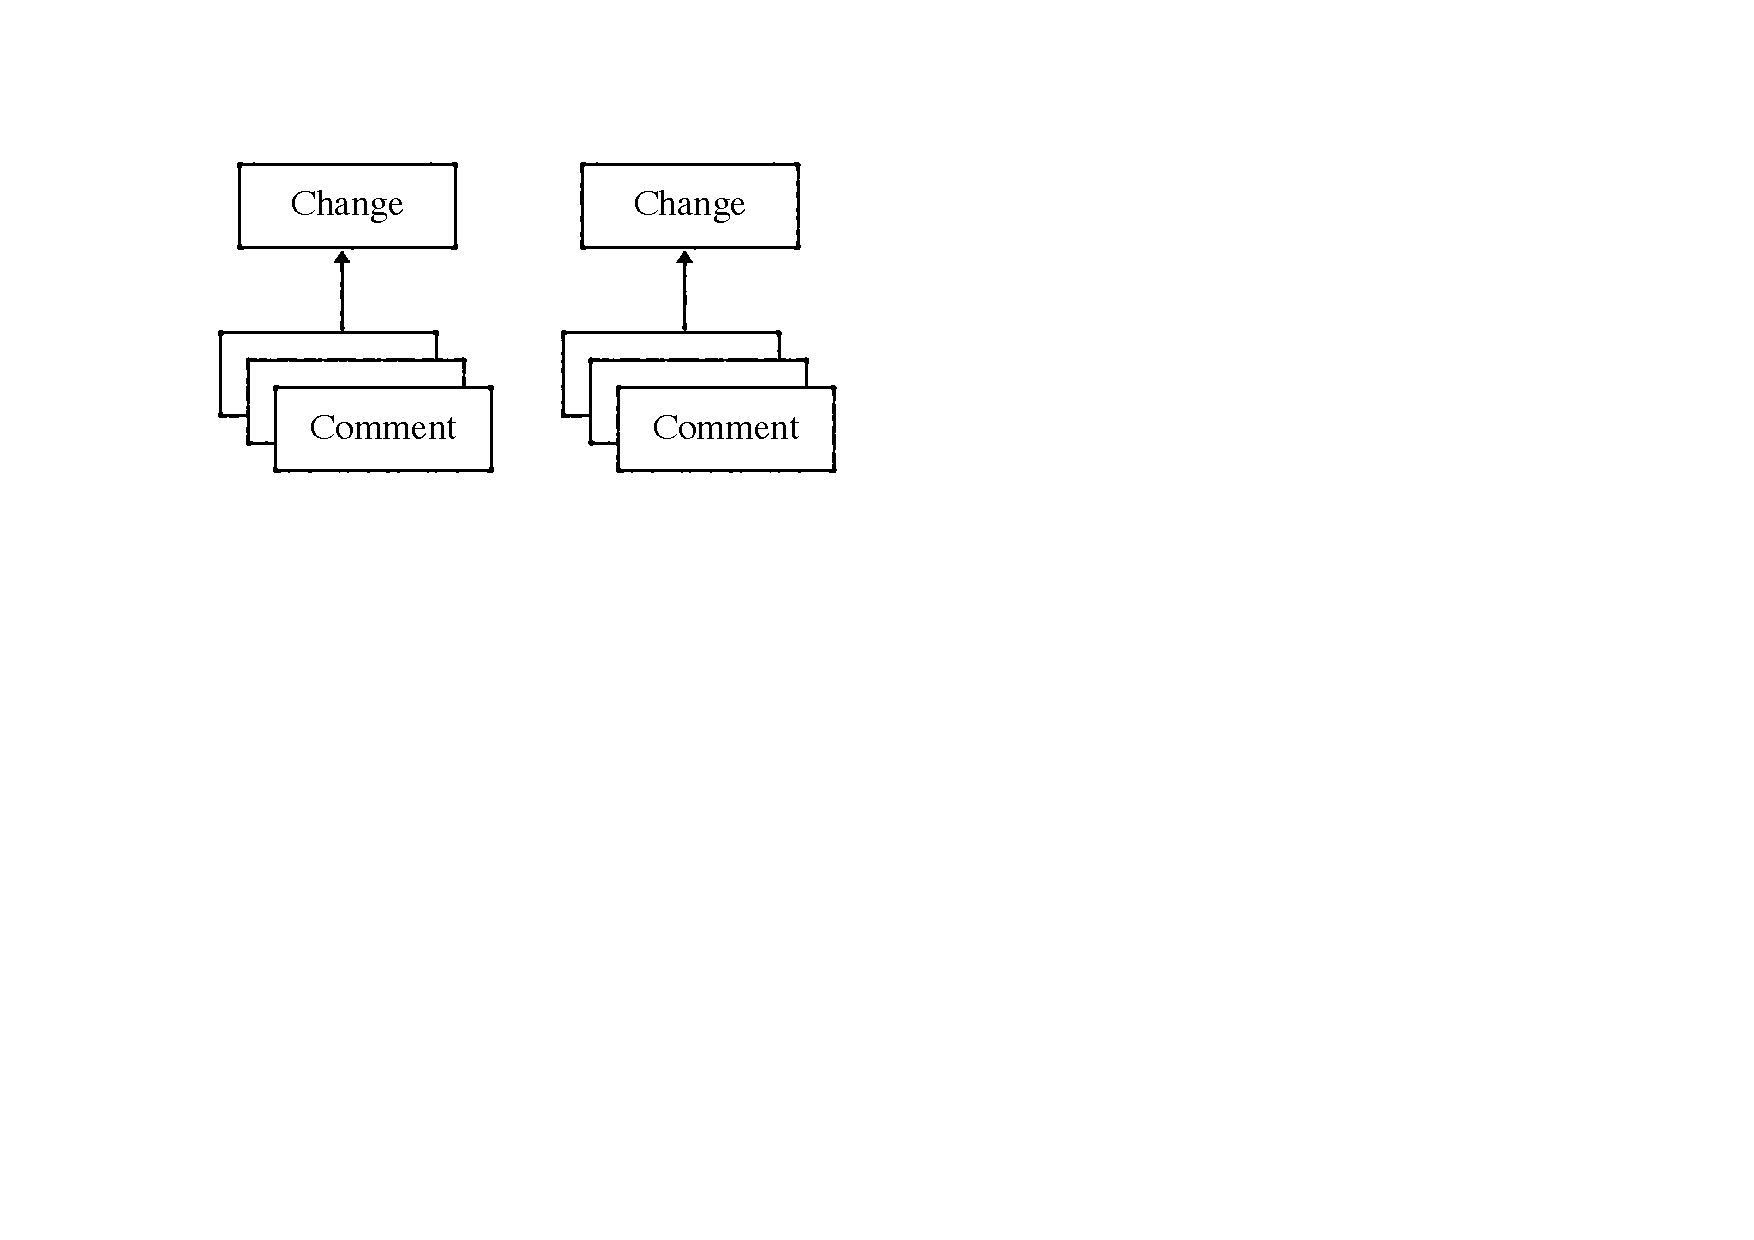
\includegraphics[width=2.5in]{hierarchy}
\caption{Relationship between documents.
Each rectangle represents a document, which may either be a commit message or a comment.}
\label{fig:hierarchy}
\end{figure}

\subsection{Data Preparation}

The commit messages and all comment texts are converted into vectors as part of the preparation step.
Fig. \ref{fig:preprocess} illustrates the overview of this step.
We wrote scripts in Ruby language to perform these tasks.

\begin{figure}[h]
\centering
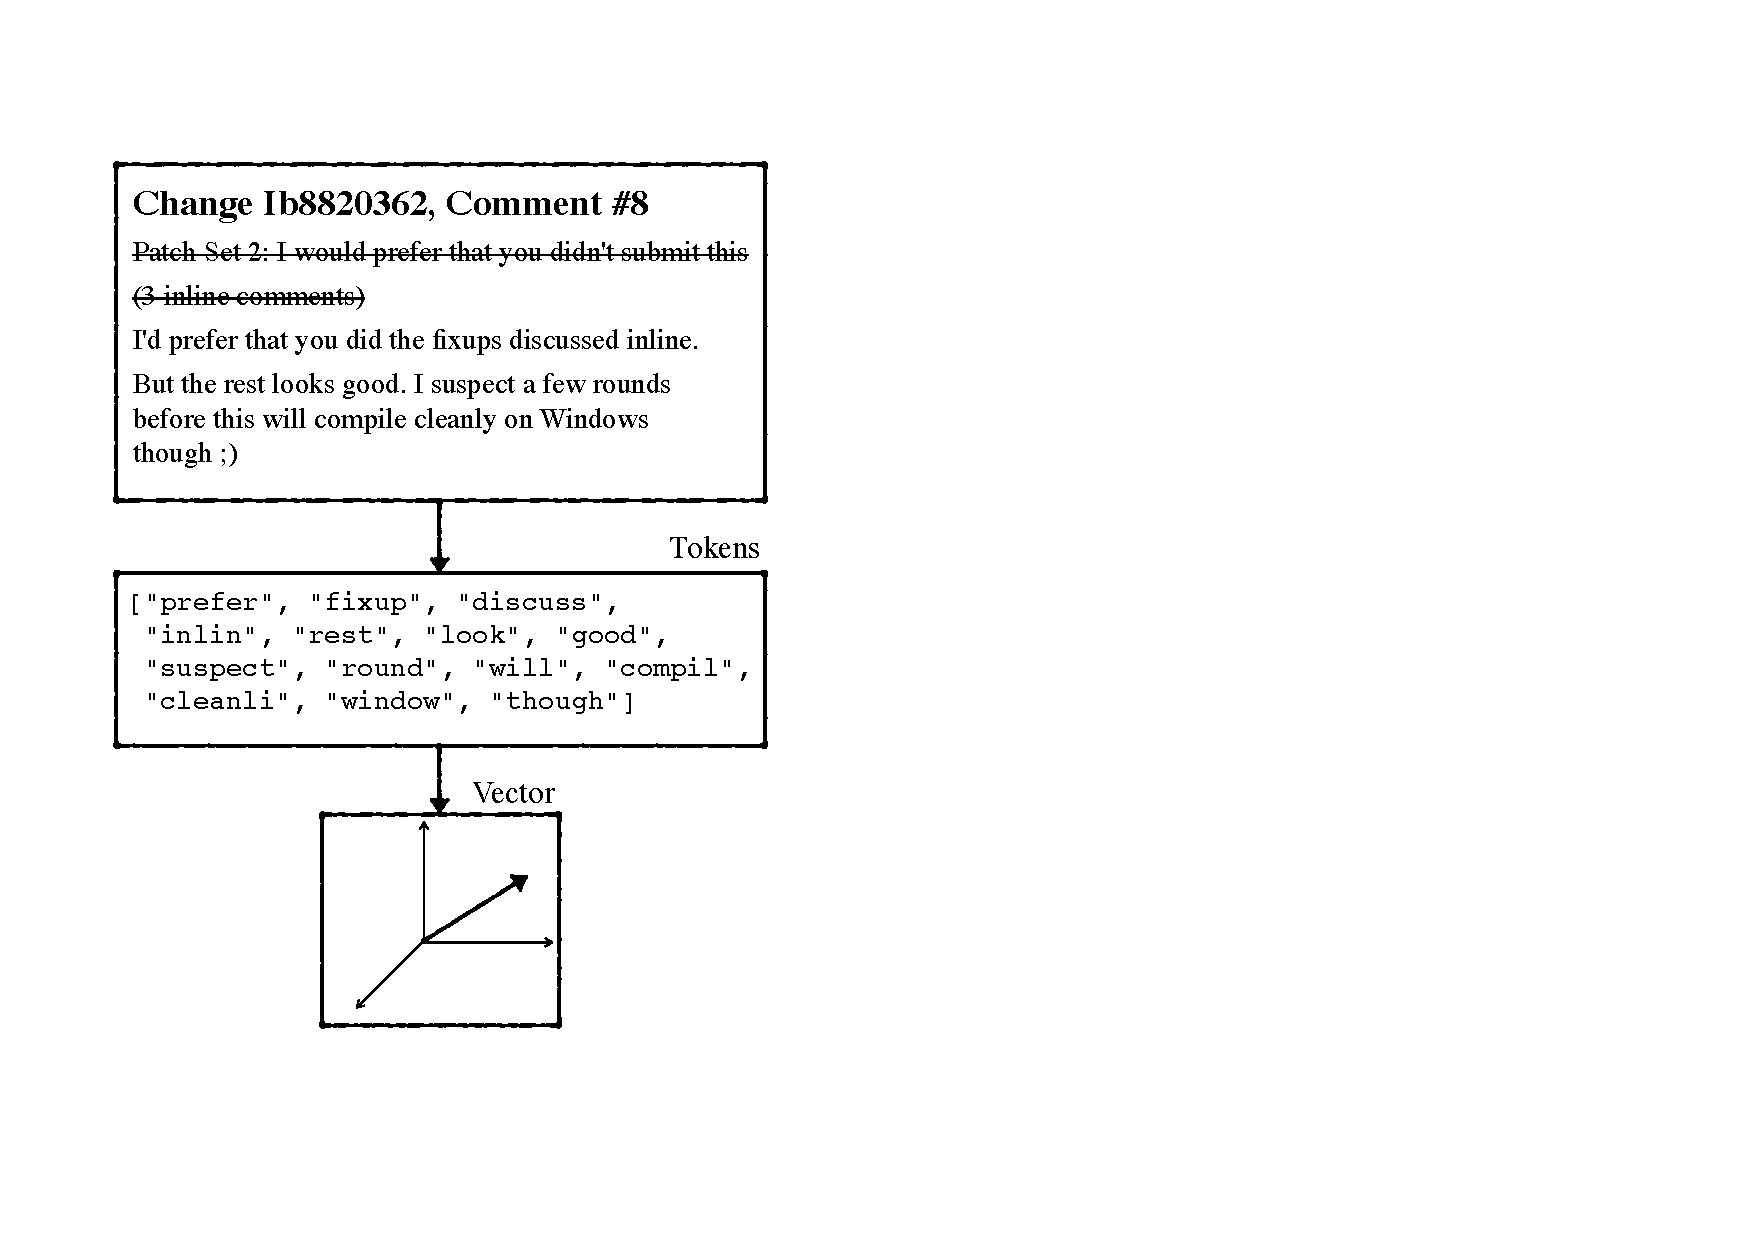
\includegraphics[width=3in]{preprocess}
\caption{The data preparation process.
Automatically generated texts are removed, remaining text is tokenized, stop words are removed, remaining tokens are stemmed,
and are converted into a vector.}
\label{fig:preprocess}
\end{figure}

\subsubsection{Removal of automatically generated text}

First, all comments by the Gerrit system, \emph{Qt Sanity Bot}, and \emph{Qt Continuous Integration System} are skipped.

% conversion into vector, wow
Next, we looked for common patterns that appeared in the comments, because it is very likely that they are automatically generated.
This is accomplished by splitting texts into lines, and for each line, searching for words that can be found in the English wordlist\footnote{The wordlist found in \texttt{/usr/share/dict/words} from Ubuntu Linux distribution is used.}.
This effectively removed the ID numbers and other non-generic terms.

Next, the lines that appears most frequently are identified.
From these lines, we then constructed the regular expression patterns,
and finally, these patterns are used to filter out automatically generated text from our data.

\subsubsection{Tokenizing, stop word removal and stemming}

After the automatically generated messages are removed, we extracted the words in each document into a list of tokens by searching for alphanumeric characters including apostrophes.
Stop words from the Google stop word list\footnote{Available at \url{http://meta.wikimedia.org/wiki/Stop_word_list/google_stop_word_list#English}} are then removed.
The stemming is performed on remaining tokens using Porter stemming algorithm.
The remaining words are then combined to form a corpus of all used words.

\subsubsection{Conversion into vector}

Finally, the tf--idf algorithm is used to convert each document into a vector.


\subsection{Training Data}

We sampled 320 comments from the data set.
These samples are then classified as either useful (that is, technically contributing to the software) or not useful.
This task is carried out by three people who worked independently.

Each comment is then scored based on the number of positive answers.
For example, a comment with a score of 3 means that all three people said that it is useful,
while a comment with a score of 0 means that none of us marked it as useful.

%The score of a comment can be defined as:

%\begin{align*}
%Score_i & = \sum_{\text{reviewer } r} Review(r, i). \\
%Review(r, i) & = \begin{cases}
%	1 & \text{if } r \text{ says that the comment } i \text{ is useful,} \\
%	0 & \text{otherwise.}
%\end{cases}
%\end{align*}

\subsection{Model Generation and Validation}

% the metrics
For each comment, we computed similarity and dissimilarity metrics
between the comment text and the corresponding commit message.
We chose cosine similarity and euclidean distance as the metrics to use in model generation.

% assumptions in categorization
The model is based on two assumptions: that useful comments will have a $similarity \geq A \text{ and } distance \leq B$,
and that comments that are not useful will have a $ similarity \leq C \text{ and } distance \geq D$,
where $A$, $B$, $C$, and $D$ are some constant.\footnote{We also tried using the `or' operator, and found that using `and' produces better result.}

% finding parameters
To find these parameters, a brute-force approach is used.
This is possible because the set of $similarity$ and $distance$ values are discrete.
Each possible value of $A$, $B$, $C$, and $D$ are evaluated to find the constant that returns the maximum F$_1$ score.

% validation
To validate our model, 10-fold cross validation is performed.
The values of precision, recall, F$_1$ score, and accuracy are recorded and then averaged
to give the overall performance of our model.


\section{Results}

\subsection{Data Preparation}

In total, there are 6,605 changes and 72,484 comments. 25,076 comments are by the system or one of the bots.

\subsubsection{Common pattern removal}

Many common patterns are found, such as \emph{`Uploaded patch set 2.'} and \emph{`Change has been successfully cherry-picked to the staging branch as \dots'}.
The occurrences of these patterns are removed from our data set.
This leaves 36,738 comments empty, which probably means that the whole comment is automatically generated.
Only 17,275 comments and commit messages are left.

\subsubsection{Tokenizing}

After preprocessing, 393,238 tokens are generated in total. They are composed of 20,025 different words.
This means that each document will be converted into a vector of 20,025 dimensions, each dimension representing a single word.



\subsection{Training Data}

After the 320 sample comments have been labeled,
they are scored based on the number of ``yes'' given to the sample.
The table below shows the distribution of scores for the training data.


\begin{center}
\begin{tabular}{|r|r|}
\hline
\bfseries Score & \bfseries Count \\
\hline
0 & 87 \\ 1 & 60 \\ 2 & 51 \\ 3 & 122 \\
\hline
\end{tabular}
\end{center}



% corpus size and other statistics



\subsection{Studied Project and Data set}
\subsection{RQ1: Can we identify useful and useless discussion in code review?}
\subsection{RQ2: How impact of useless discussion impact to the software quality?}


\section{Discussion}



\section{Threat to Validity}


\section{Conclusion and Future Work}


\IEEEpeerreviewmaketitle

\bibliographystyle{IEEEtran}

\bibliography{references}



% that's all folks
\end{document}


